\documentclass[12pt,a4paper,titlepage]{article}
\title{Simulations of Monolayer and Multilayer MoS$_2$ FET} 
\author{Matteo Orlandini \& Jacopo Pagliuca}
\date{}

\usepackage[italian, english]{babel} %the last declared language is the one used in the document
\usepackage[utf8]{inputenc}
\usepackage[T1]{fontenc}
\usepackage{amsmath}
\usepackage{amssymb}
\usepackage{subfig}
\usepackage{graphicx}
\usepackage{listings}
%inizio impostazioni bibliografia
\usepackage[autostyle,italian=guillemets]{csquotes} 
%autostyle adatta lo stile delle citazioni alla lingua corrente del documento;
%italian=guillemets racchiude automaticamente tra virgolette caporali
%i campi che prevedono le virgolette;
\usepackage[backend=biber, style=numeric, citestyle=numeric,maxcitenames=99,maxbibnames = 99]{biblatex}
%backend=biber dice a biblatex che s’intende usare Biber come motore bibliografico
%style:numeric Anno di pubblicazione: in fondo al riferimento.
%citestyle=numeric Riferimento: numerico ([1], [2], eccetera).
%fine impostazioni bibliografia

\usepackage{float}
\usepackage{hyperref}
\hypersetup{
	bookmarks=true,         % show bookmarks bar?
	unicode=false,          % non-Latin characters in Acrobat’s bookmarks
	pdftoolbar=true,        % show Acrobat’s toolbar?
	pdfmenubar=true,        % show Acrobat’s menu?
	pdffitwindow=false,     % window fit to page when opened
	pdfstartview={FitH},    % fits the width of the page to the window
	%pdftitle={Relazione di Reti di Sensori Wireless per IOT},    % title
	pdfauthor={Matteo Orlandini},     % author
	pdfsubject={Simulations of Monolayer and Multilayer MoS$_2$ FET}  % subject of the document
	pdfcreator={Matteo Orlandini},   % creator of the document
	%pdfproducer={Producer}, % producer of the document
	pdfpagemode={UseOutlines},
	%bookmarksopen,
	pdfpagelabels=true
	pdfstartview={FitH},
	colorlinks=false,       % false: boxed links; true: colored links
	linkcolor={red},
	citecolor={green},
	urlcolor={cyan},
} 


\addbibresource{Bibliography.bib}

\newcommand{\CoverName}{Cover}

\begin{document}
\renewcommand{\thepage}{\CoverName}
\begin{titlepage}
	
	\centering
	\includegraphics[width=.2\textwidth]{Immagini/univpmlogo}\par\vspace{1cm}
	{\scshape\LARGE Università Politecnica delle Marche\par}
	\vspace{1cm}
	{\scshape\Large Multiphysics Systems for Radio Frequency Electronics\par}
	\vspace{1.5cm}
	{\huge\bfseries  Simulations of Monolayer and Multilayer MoS$_2$ FET \par}
	\vspace{2cm}
	{\Large\itshape Matteo Orlandini \par}
	{\Large\itshape Jacopo Pagliuca\par}
	\vfill
	supervised by\par
	Prof. Davide \textsc{Mencarelli}, Prof. Luca \textsc{Pierantoni}\\ and Nicola \textsc{Pelagalli}
	
	\vfill
	
	% Bottom of the page
	{\large \today\par}
\end{titlepage}

\thispagestyle{empty}
\pagenumbering{roman}
\tableofcontents

\newpage
\pagenumbering{arabic}
\setcounter{page}{1}
\section{Introduction}

\begin{figure}[H]
	\centering
	\includegraphics[width=1\textwidth]{Grafici/monolayer_Id(Vd).eps} 
	\label{fig:monolayer_Id(Vd))}
	\caption{Monolayer $I_d(V_d)$}
\end{figure}

\begin{figure}[H]
	\centering
	\includegraphics[width=1\textwidth]{Grafici/monolayer_Id(Vg).eps} 
	\label{fig:monolayer_Id(Vg))}
	\caption{Monolayer $I_d(V_g)$}
\end{figure}

\begin{figure}[H]
	\centering
	\includegraphics[width=1\textwidth]{Grafici/4layer_Id(Vd).eps} 
	\label{fig:4layer_Id(Vd)}
	\caption{4 layer $I_d(V_d)$}
\end{figure}

\begin{figure}[H]
	\centering
	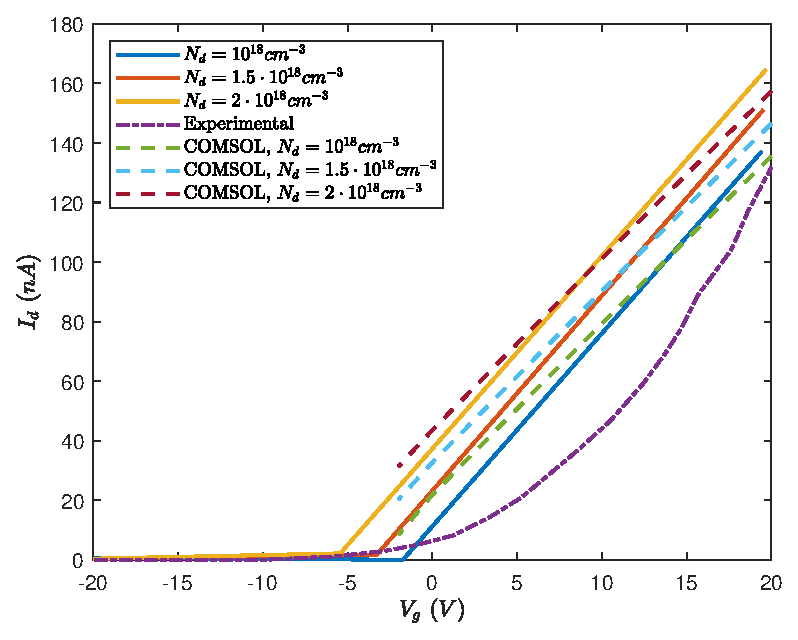
\includegraphics[width=1\textwidth]{Grafici/4layer_Id(Vg).eps} 
	\label{fig:4layer_Id(Vg)}
	\caption{4 layer $I_d(V_g)$}
\end{figure}

\begin{figure}[H]
	\centering
	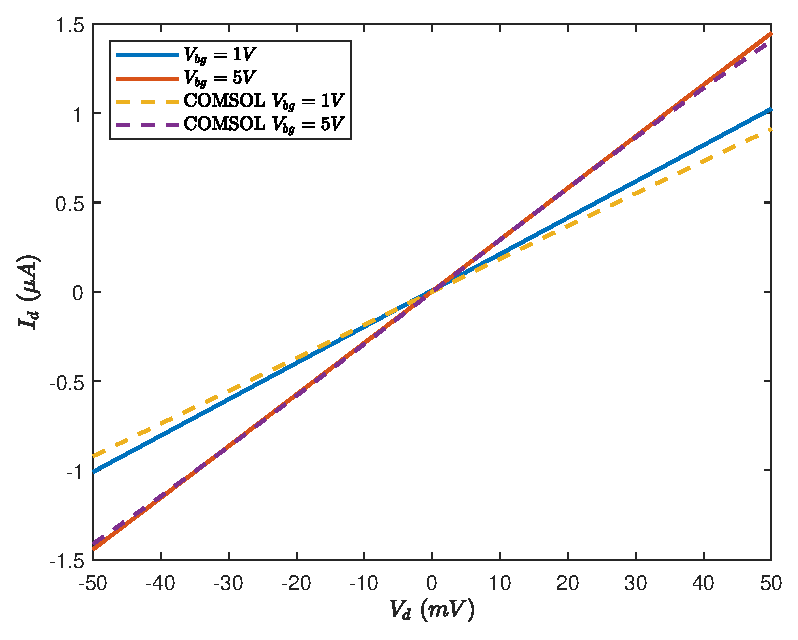
\includegraphics[width=1\textwidth]{Grafici/Id(Vd)_HfO2_MoS2.eps} 
	\label{fig:Id(Vd)_HfO2_MoS2}
	\caption{$I_d(V_d)$}
\end{figure}

\begin{figure}[H]
	\centering
	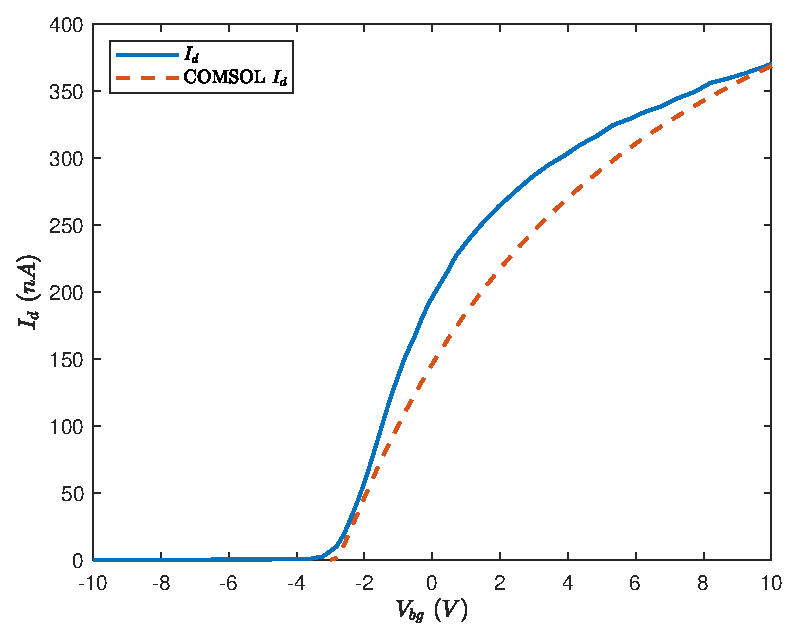
\includegraphics[width=1\textwidth]{Grafici/Id(Vbg)_HfO2_MoS2.eps} 
	\label{fig:Id(Vbg)_HfO2_MoS2}
	\caption{$I_d(V_{bg})$}
\end{figure}

\begin{figure}[H]
	\centering
	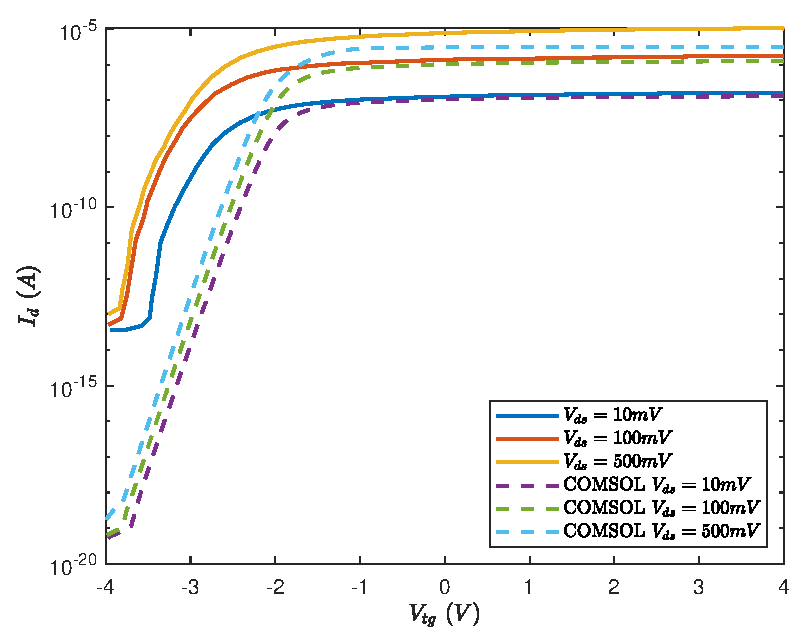
\includegraphics[width=1\textwidth]{Grafici/Id(Vtg)_HfO2_MoS2_varying_Vds.eps} 
	\label{fig:Id(Vtg)_HfO2_MoS2_varying_Vds}
	\caption{$I_d(V_{tg})$ varying $V_{ds}$}
\end{figure}

\begin{figure}[H]
	\centering
	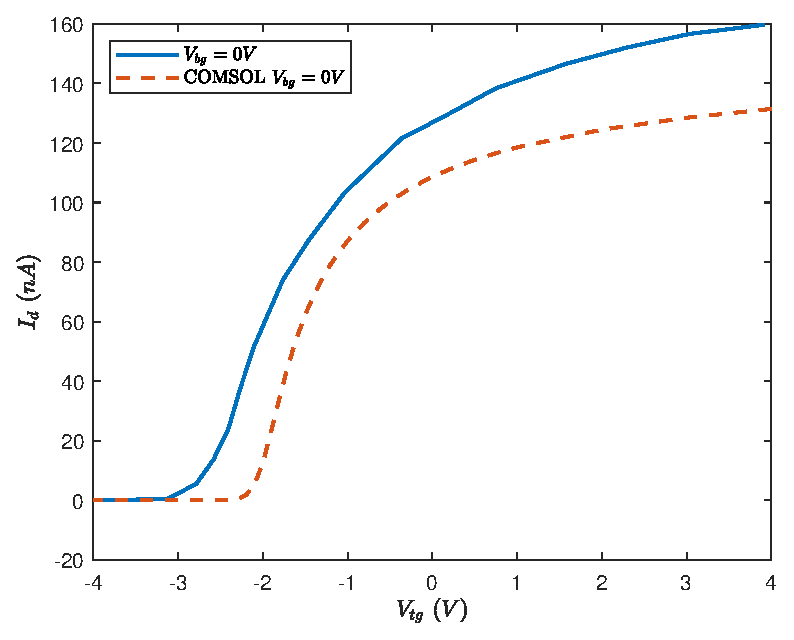
\includegraphics[width=1\textwidth]{Grafici/Id(Vtg)_HfO2_MoS2_varying_Vbg.eps} 
	\label{fig:Id(Vtg)_HfO2_MoS2_varying_Vbg}
	\caption{$I_d(V_{tg})$ varying $V_{bg}$}
\end{figure}

\begin{figure}[H]
	\centering
	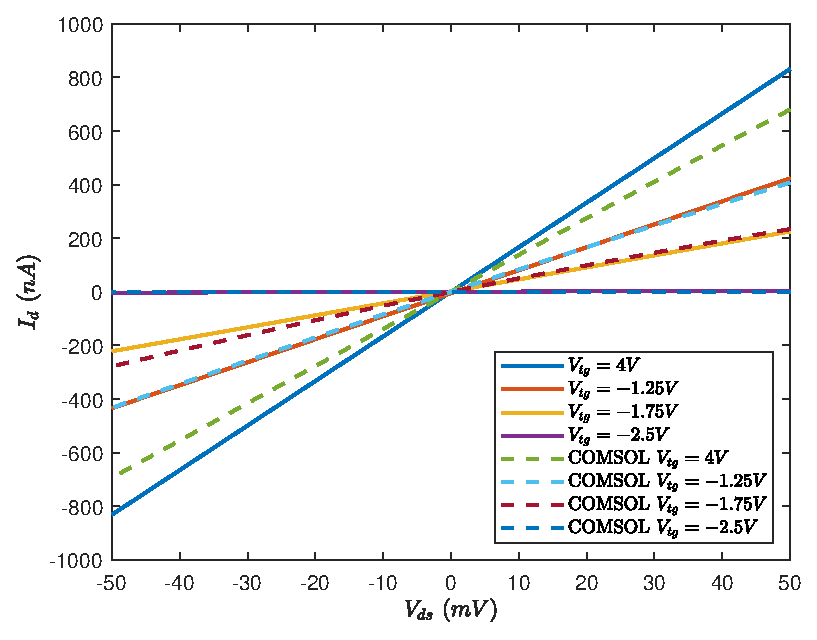
\includegraphics[width=1\textwidth]{Grafici/Id(Vds)_HfO2_MoS2_varying_Vtg.eps} 
	\label{fig:Id(Vds)_HfO2_MoS2_varying_Vtg}
	\caption{$I_d(V_{ds})$ varying $V_{tg}$}
\end{figure} 

\newpage

\nocite{*}
%Il comando \printbibliography produce la sezione bibliografica con relativi
%titolo e testatina. Per mandarne il relativo titolo nell’indice generale si
%usa l’istruzione:
\printbibliography

\end{document} 